\section{Conclusions}

The results presented in this work provide the first tests and verification of the digital back-end for novel readout technology targeted at liquid Argon Time-Project-Chambers.

The first Q-Pix analog prototype using Off-The-Shelf analog components has been built and is currently taking measurements.
This prototype promises to provide gaseous Argon diffusion measurements, which will likely be the first true physics measurement using a Q-Pix based readout.

We have built and verified the first digital prototype boards which have verified communication reliability to protect against potential data loss.
We developed a frequency calibration method for remote nodes to demonstrate Q-Pix's ability to have independent oscillators.
We used this prototype and verified the ability to reconstruct remote oscillator frequencies with a precision more than an order of magnitude required (0.1~\unit{ppm} < 1~\unit{ppm}).
These results are verified between two different interrogation frequencies.

We developed multiple simulations to model the detector's response to long ($1000 second$) run time exposure of radiogenic backgrounds as well as tested the ability to readout beam neutrino events at LBNF.
Our simulations show that the current FIFO local (64) and remote (128) depths of the digital ASIC prototype are too small.
We estimate that the local FIFO depth should be at least be able to record 426 unique resets in order to fully capture 99\% of neutrino events with energy up to 10~\unit{GeV}.
This result provides the first limit on the memory required for a Q-Pix ASIC, should it be used in a DUNE-FD module to measure neutrino oscillations.

To test the remote FIFO and frequency requirements we developed the first simulation to model the Q-Pix digital back-end response to physical events within a DUNE-FD APA.
We find that the distribution of the ASIC frequency needs to be $\approx 0.5\%$ in order to maintain obtain reliable remote FIFO depths with the current readout method. 
These results also indicate that the only reliable routing methodolgy is the "Snake" routing (Section~\ref{sec:}), which is independent of both tile size and digital architecture.
This routing ("Snake") provides a unitary relationship between the local and remote FIFO depth requirements.

\subsection{The Future of Q-Pix}

The Q-Pix design is a novel readout technology.
However, "novelty does not confer automatically benefit", David Nygren.
The full Q-Pix validation still awaits key results to demonstate its capabilities in a DUNE-FD module.
Namely, Q-Pix still needs to test both the analog and digital prototypes at cold liquid Argon temperatures.

The front-end requires a reliable replenishment circuit as well as low leakage current ($\approx 100~\unit{aA}$ or less to be below radiogenic backgrounds).
Also, the limitation of the timing from the replenishment circuit should be applied to the RTD results presented in this work.
The combination of the timing response of the analog front-end along with the neutrino simulation events here will allow accurate event reconstruction.
With these reconstructed events in hand analysis can proceed to estimate of Q-Pix's ability to perform neutrino oscillation measurements.

\subsection{Q-Pix's First and Second Digital Prototypes}

The work presented here can accurately be viewed both as a means to understand the Q-Pix's first digital ASIC and as a guide to the second digital design.
The key result of this work indicates that the local and remote FIFO depths of the second prototype should both be increased to at or above 426.
The reason the first prototype did not incorporate these larger buff sizes to begin with was due to fabrication limitiations of the ASIC.
If oscillator tests of the first prototype indicate that the mean drift between neighbor ASICs is reliably under 0.5\%, then the local oscillator need not be changed either.
All other underlying logic, with perhaps the exception of FWFT FIFOs, have been verified in the first digital prototype.
These tests need only be repeated on the first prototype ASIC.

Eventually the Q-Pix front and back-end ASICs will likely be combined into a single chip.
Still, the motivation provided by the results presented here for the second prototype (applied only to the digital portion) remain unchanged.

\section{Future Neutrino Oscillation Studies}

Although an analysis of the reconstruction of the events involving oscillation are slightly beyond the scope of the work presented here, we provide a brief summary of how the work presented may be applied to that analysis.
The LBNF beam flux, neutrino oscillations, and neutrino cross-sections all affect the neutrino event rate as a function of energy.
Instead of applying these factors, we tested against a uniform distribution of neutrino interaction energy.

Figure~\ref{fig:energy_deposit_vs_resets} clearly shows the relationship between the energy deposited and the number of resets collected.
To account for neutrino oscillation and appearance probability as a function of energy, we would weight the buffer depths based on the weights for the different neutrino flavors as shown in Figures~\cref{fig:electron_interaction,fig:muon_interaction}.
However for both flavor of (anti)neutrino, the peak of the distribution is below 5~\unit{GeV}.

\begin{figure}[]
\centering
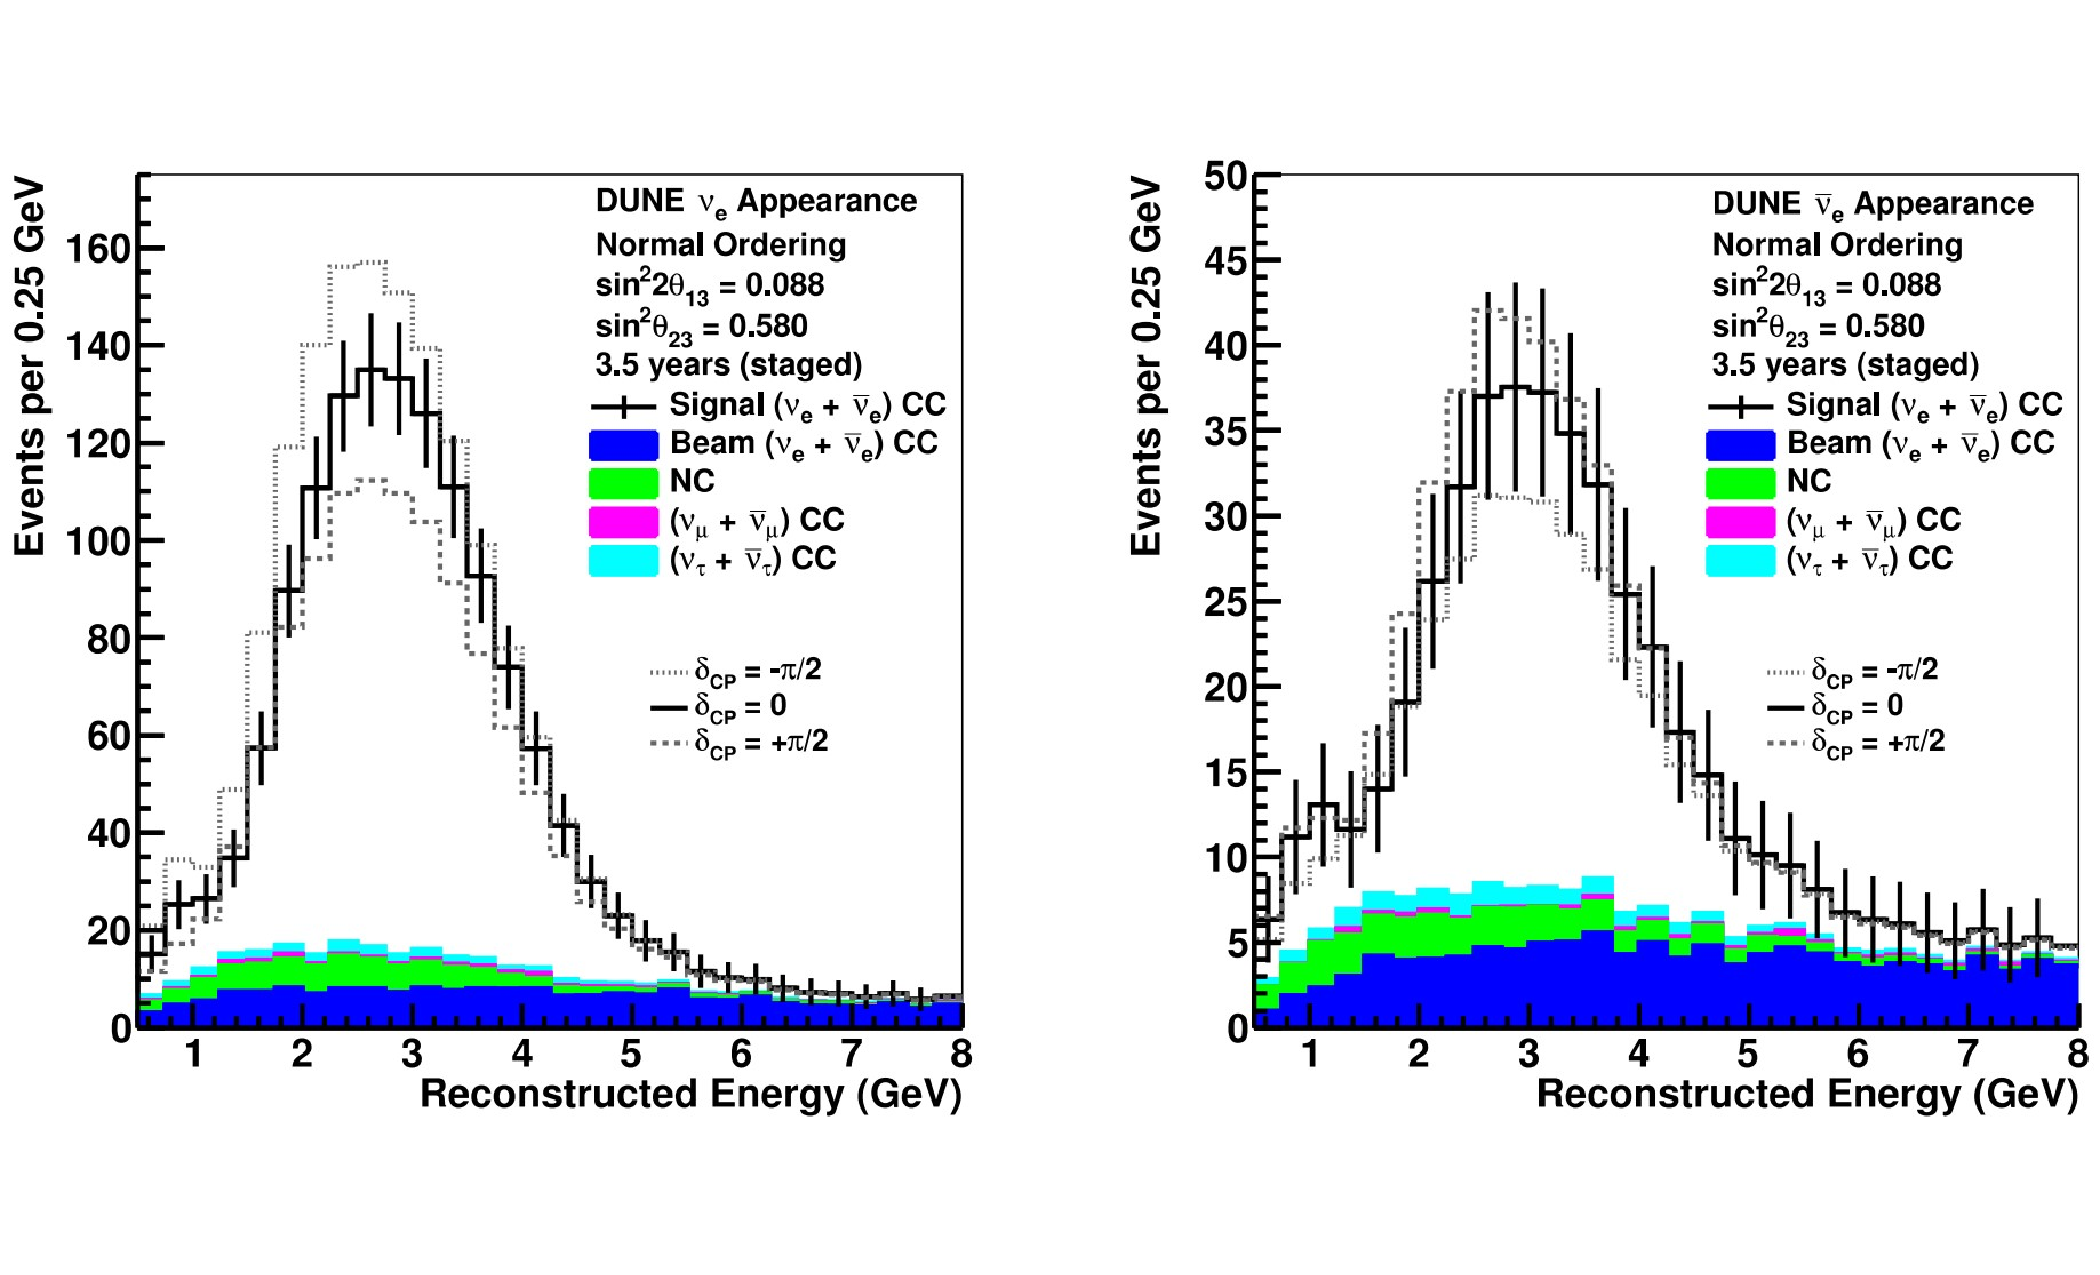
\includegraphics[width=\textwidth]{images/tdr_electron_reconstruction_tdrv2.pdf}
\caption{Figure is taken from from the DUNE-FD TDR~\citep{DUNE_FD_TDRv2_2020}.
Images show the $\nu_{e}$ and $\bar{\nu_{e}}$ appearance spectra respectively.
The left image shows the reconstructed energy distribution for the beam running in the forward horn current direction for 3.5 years.
The weight of appearance spectra decreases with increasing energy beyond $\approx 8~\unit{GeV}$ and has a maximum between 1 and 2~\unit{GeV}.
}
\end{figure}~\label{fig:electron_interaction}

\begin{figure}[]
\centering
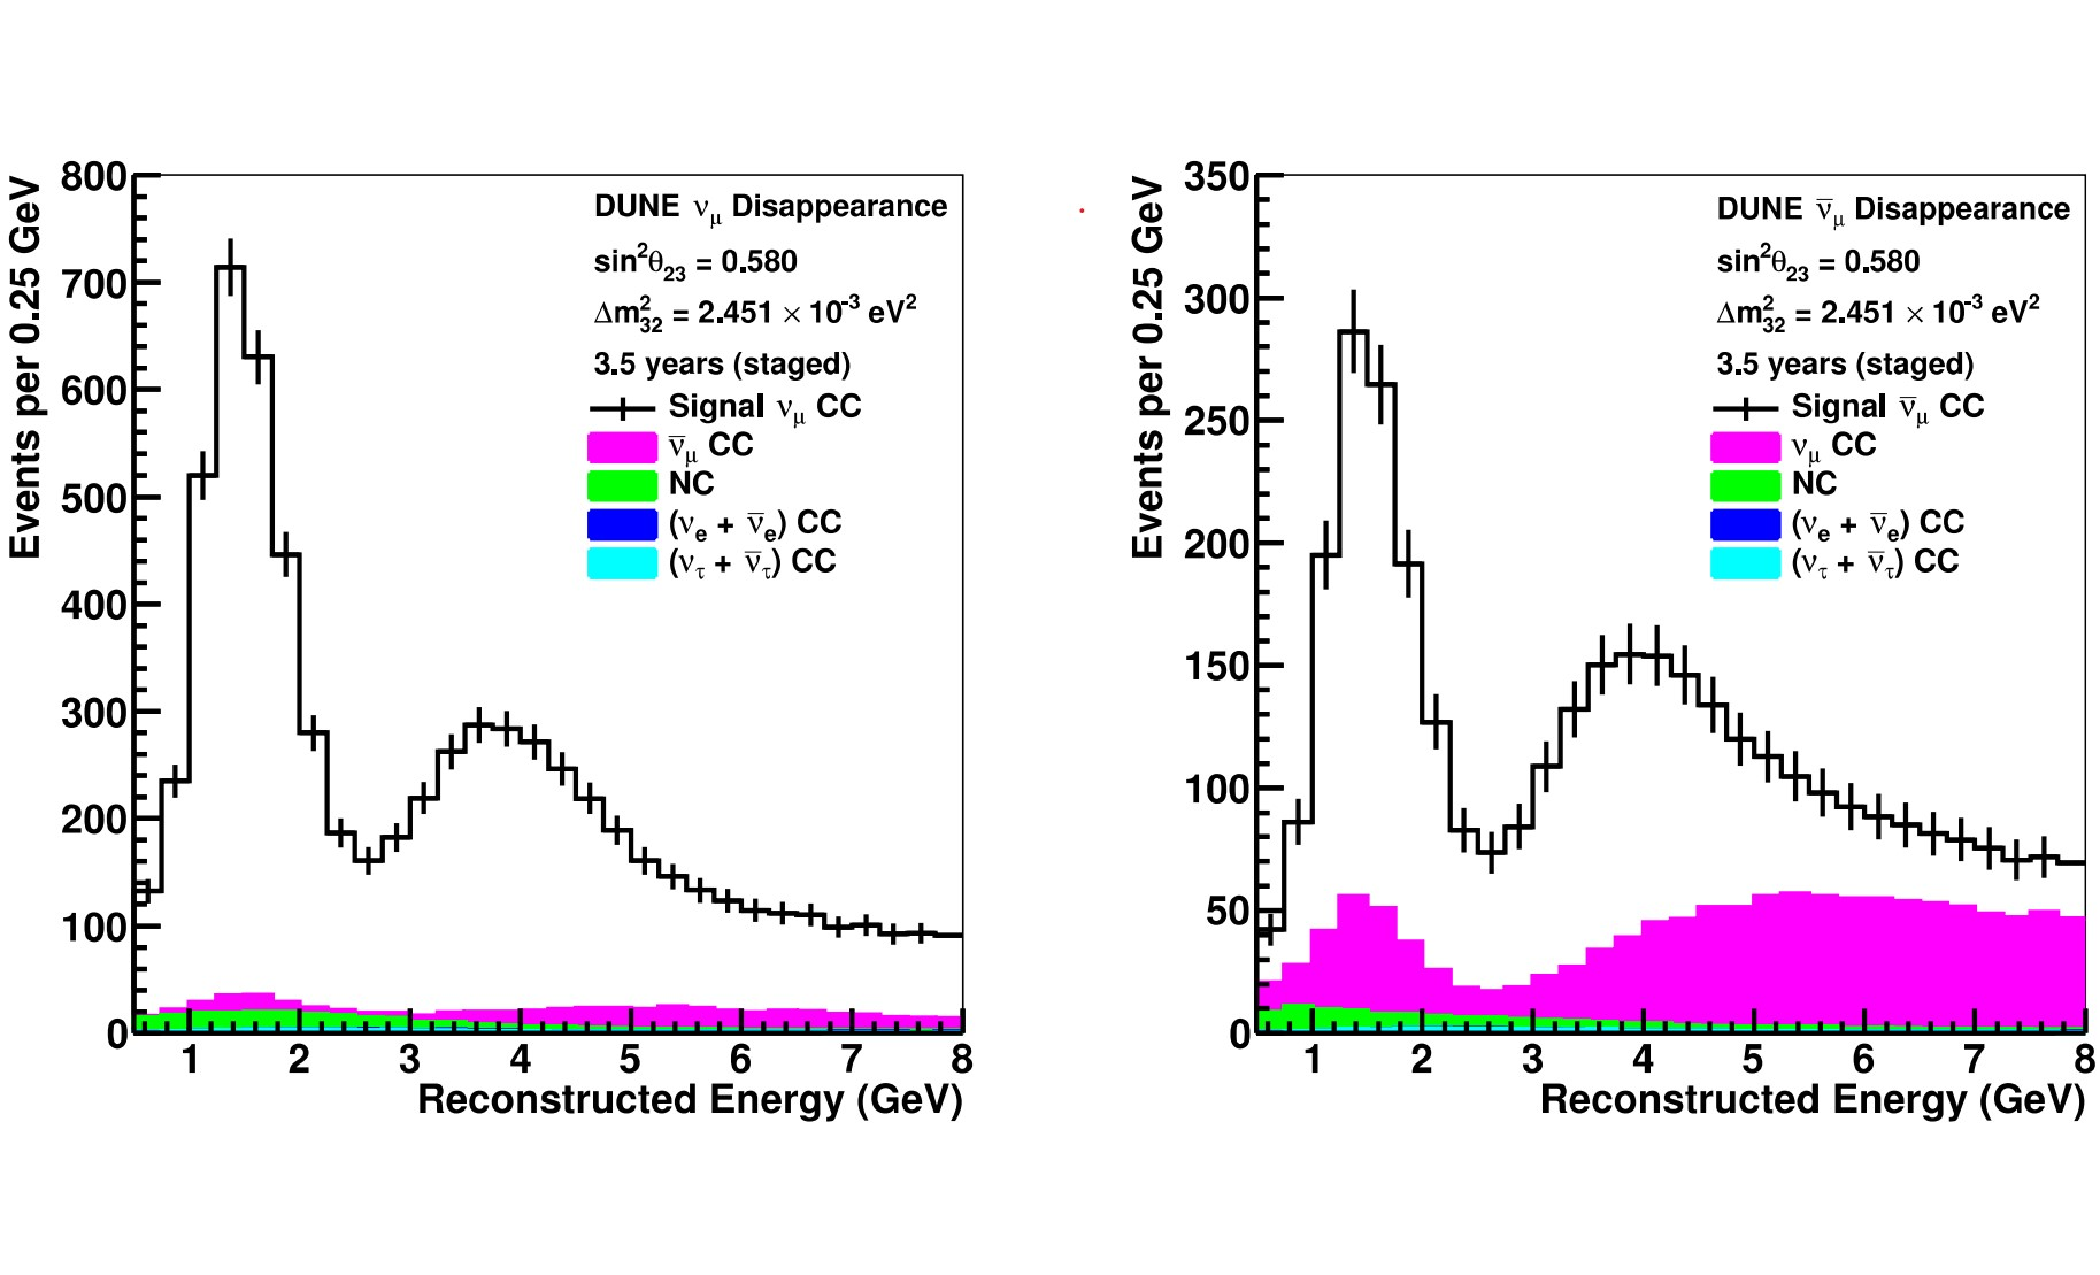
\includegraphics[width=\textwidth]{images/tdr_muon_reconstruction_tdrv2.pdf}
\caption{Figure is taken directly from the DUNE-FD TDR~\citep{DUNE_FD_TDRv2_2020}.
Images show the $\nu_{\mu}$ and $\bar{\nu_{\mu}}$ disappearance spectra respectively.
The plots assume normal mass ordering and are also stagged for 3.5 years (staged) exposure for the beam running in the forward horn current and 7 years in the reverse horn current.
The weight of disappearance spectra decreases with increasing energy beyond $\approx 8~\unit{GeV}$ and has a maximum between 1 and 2~\unit{GeV}.
}
\end{figure}~\label{fig:muon_interaction}

The analysis presented here uses a uniform distribution of true neutrino energy up to 10~\unit{GeV} and therefore over estimates the average energy deposited.

\begin{figure}[]
\centering
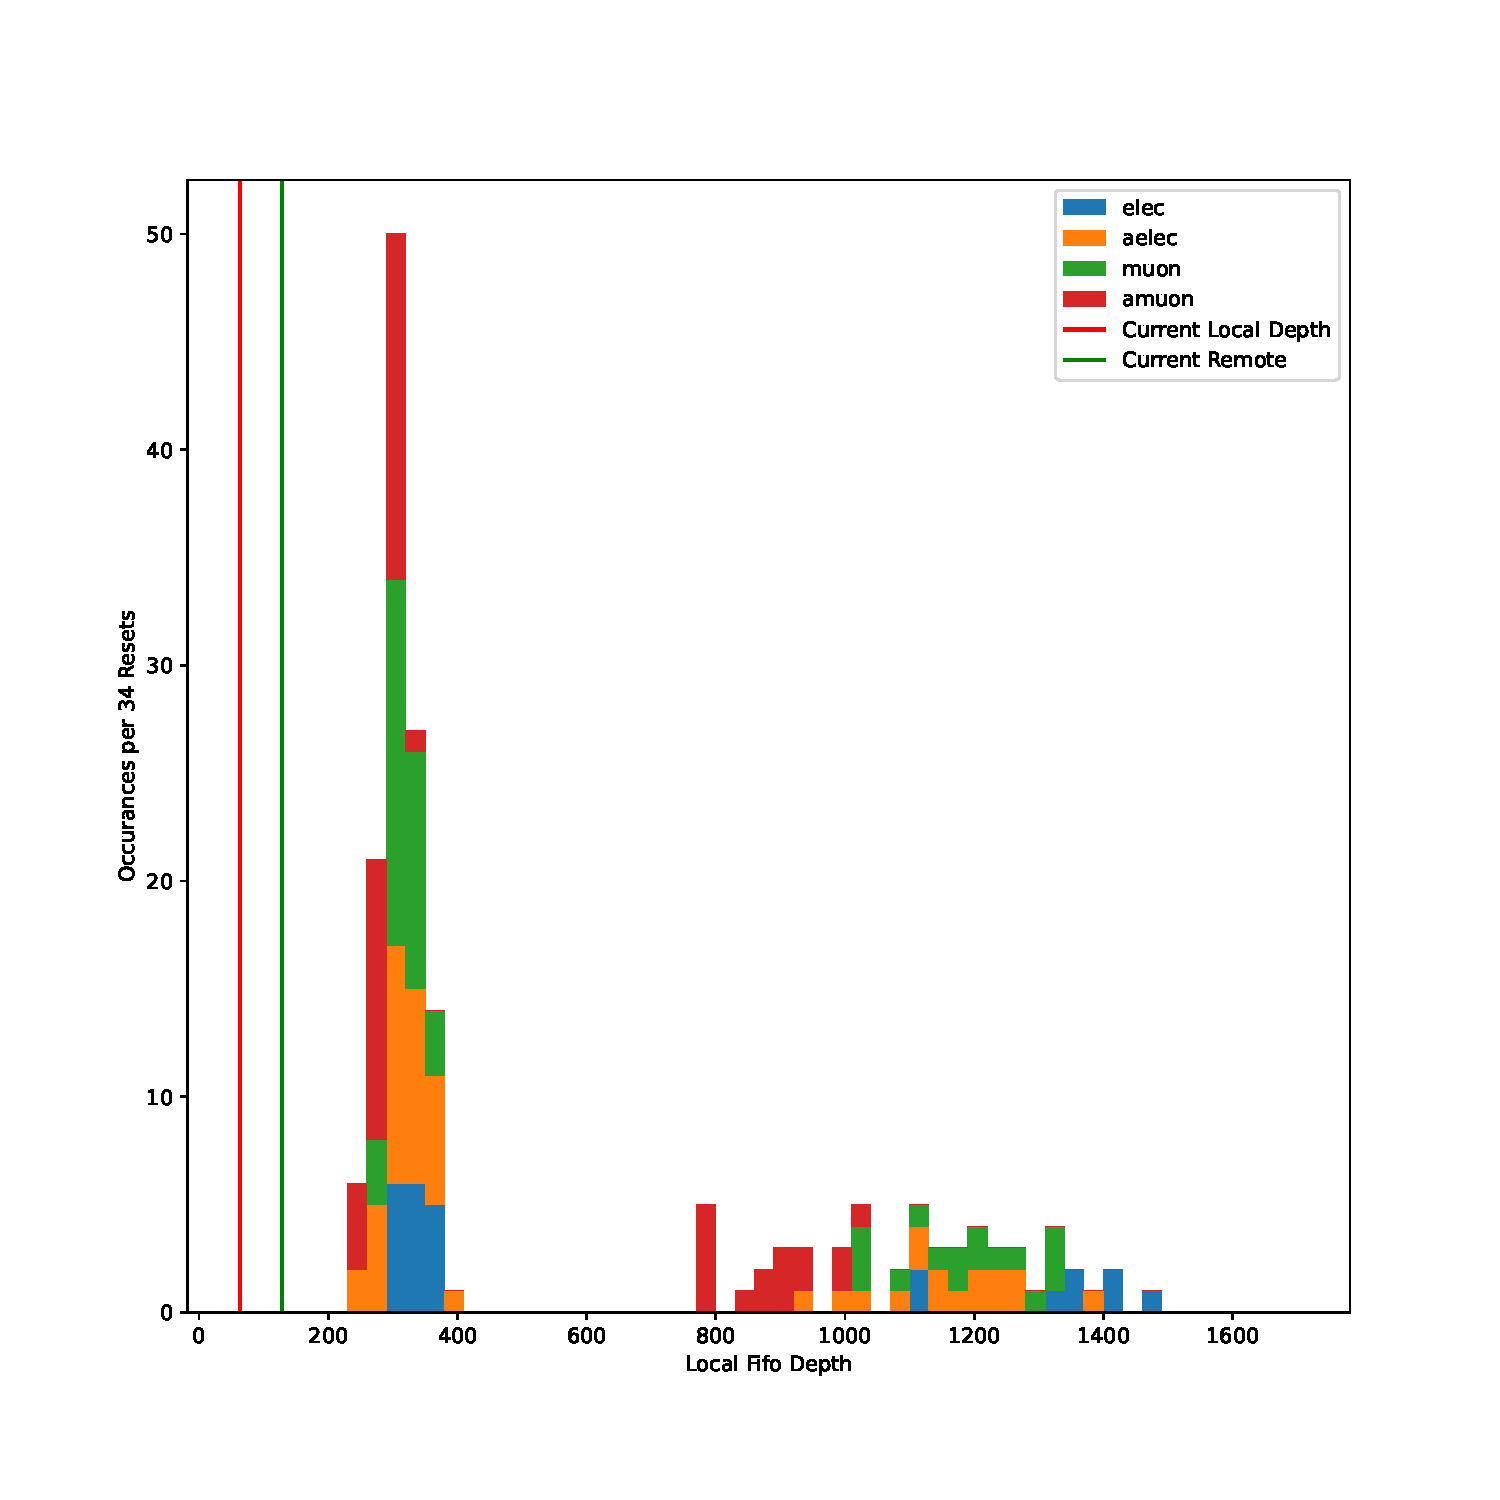
\includegraphics[width=\textwidth]{images/df_weight_pdg_cut.pdf}
\caption{Weighted integrals for all neutrino event parameters, with weights drawn from the expected signal curves from Figure~\ref{fig:electron_interaction} and Figure~\ref{fig:muon_interaction}.}
\end{figure}~\label{fig:weighted_integrals}